\documentclass{report}
\usepackage[utf8]{inputenc}
\usepackage{graphicx}
\usepackage{amssymb}

\title{Introduzione}
\author{Matteo Cerinelli}
\date{10 Luglio 2024}

\begin{document}

\maketitle

\section*{Prova}

In questa sezione viene presentata una panoramica generale dell'argomento trattato nel presente documento. 
Verranno illustrate le motivazioni che hanno portato allo sviluppo di questo lavoro, gli obiettivi prefissati e la struttura del testo. 
L'introduzione ha lo scopo di fornire al lettore il contesto necessario per comprendere le tematiche affrontate nei capitoli successivi.



\section{Recap Appunti}

In questa sezione si fornisce un breve riassunto degli appunti presi durante le lezioni.


\begin{center}
    \label{dataset}
    \textbf{Figura 1:} Esempio di dataset utilizzato per l'analisi.\\
    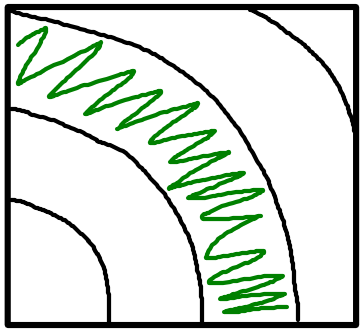
\includegraphics[width=0.3\textwidth]{./Pictures/EsempioDataset.png}
    
    Nella striscia verde dovrebbero essere tutte della stessa famiglia\\
    Vedremo che sono diversi in base al \textit{Gene di espressione}.\\
    Il gene lo capiamo dal DNA
\end{center}


Un gene può essere acceso, spento e/o regolato \textrightarrow \space quantità di RNA prodotto

\newpage
\begin{center}
    \textbf{Figura 2:} Come dovrebbe essere.\\
    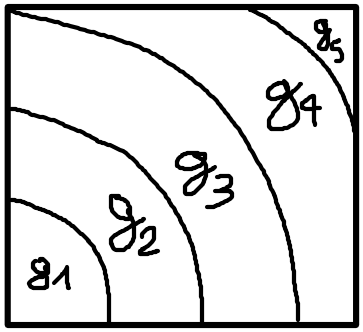
\includegraphics[width=0.3\textwidth]{./Pictures/ComeDovrebbeEssere.png}
    
    Il gene deve seguire i confini, ma succede però che ci sono alcuni geni strani, Ovvero a cavallo tra due zone!\\
    \textbf{Vanno tolti!}\\
\end{center}

\begin{center}
    Voglio capire i geni che sono simili e capire se ci sono \textit{cluster spaziali}\\

    \textbf{Figura 3:} Capire quali cluster cozzano!\\
    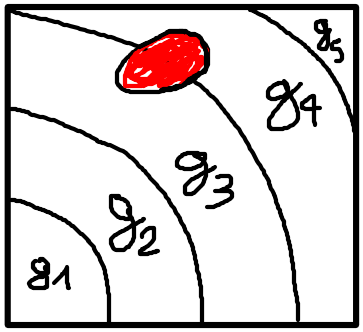
\includegraphics[width=0.3\textwidth]{./Pictures/Cozzano.png}

    Vediamo che g6 (rosso) interseca con g4 e g3
\end{center}

\section*{ToDo}
Informarsi bene su questi argomenti:
\begin{itemize}
    \item \textbf{SVGs}: Spatially Variable Genes
    \item \textbf{HVGs}: Highly Variable Genes

\end{itemize}

\subsection{SVGs}
Sono i geni che mostrano una variabilità espressionale particolarmente alta tra le cellule, superiore a quella attesa data la loro media di espressione.\\
Si usano spesso per clusterizzare le cellule.
\subsection{HVGs}
Sono i geni che mostrano variazioni di espressione associate alla posizione spaziale nel tessuto.
\renewcommand{\labelitemi}{\checkmark}
\begin{itemize}
    \item Capire l’architettura spaziale del tessuto
    \item Identificare domini o regioni funzionali.
\end{itemize}

\chapter*{Abstract}
\label{chap:abstract}
\subsection*{Cosa è il DNA}

Il \textbf{DNA}\footnote{È fatto da una doppia elica formata da nucleotidi (A, T, C, G)} è il manuale di istruzioni della cellula, contiene le informazioni necessarie per la sintesi delle proteine e per il funzionamento della cellula stessa.
Ogni cellula ha lo stesso DNA.\\
Un \textbf{Gene} è una porzione di DNA che contiene le istruzioni per la sintesi di una proteina.\\

\subsection*{Cosa è l'RNA}
L'\textbf{RNA} è una molecola che trasporta le informazioni genetiche dal DNA ai ribosomi, dove avviene la sintesi delle proteine.\\

\subsection*{Cosa è la Trascrittomica}
La \textbf{Trascrittomica}\footnote{Utile per capire quali geni sono attivi e in che quantità} studia tutti gli RNA messaggeri prodotti da una cellula o un tessuto in un certo momento.\\
La \textbf{Trascrittomica Spaziale} si occupa di studiare l'espressione genica in un contesto spaziale, ovvero come i geni sono espressi in diverse regioni di un tessuto.\\


\end{document}